\section{Εισαγωγή}

\subsection{Ταυτότητα - επιχειρησιακοί στόχοι}

Σκοπός της ομάδας saiko-killers είναι η δημιουργία μιας ενιαίας πλατφόρμας που ενθαρρύνει τη συνεργατική παρατήρηση τιμών πρατηρίων υγρών καυσίμων και παρέχει αυτές τις πληροφορίες δωρεάν σε κάθε χρήστη. Καθώς τα υγρά καύσιμα αποτελούν βασικό και απαραίτητο αγαθό της σύγχρονης δυτικής κοινωνίας θεωρείται αρκετά πιθανό το παραπάνω σύστημα να προσεγγίσει μεγάλο μέρος πληθυσμού γεγονός που μπορεί να μεταφραστεί ως κέρδος για τους διαχειριστές του συστήματος μέσα από μελλοντικές διαφημιστικές προωθήσεις.

\subsection{Περίγραμμα επιχειρησιακών λειτουργιών}

Ο διαχειριστής της ιστοσελίδας εχει τη δυνατότητα να κάνει sign in με συγκεκριμένα στοιχεία διαχειριστή προκειμένου να έχει ασφαλή πρόσβαση στο backend της εφαρμογής.
Μετά την επιτυχή σύνδεση ο διαχειριστής θα βλέπει τους εγγεγραμμένους χρήστες του συστήματος και τα καταχωρημένα πρατήρια υγρών καυσίμων.

Ο διαχειριστής θα μπορεί να πραγματοποιεί: 
\begin{enumerate}
	\item Ανάθεση/ανάκληση ρόλων καθώς και κλείδωμα χρήστη
	\item Εισαγωγή/διαγραφή πρατηρίων από τη βάση δεδομένων
	\item Γενική επισκόπηση δεδομένων συστήματος
	
\end{enumerate}

Η παραπάνω συμπεριφορά μοντελοποιείται στο διάγραμμα δραστηριοτήτων UML του σχήματος  \ref{admin}.

\begin{figure}
	\centering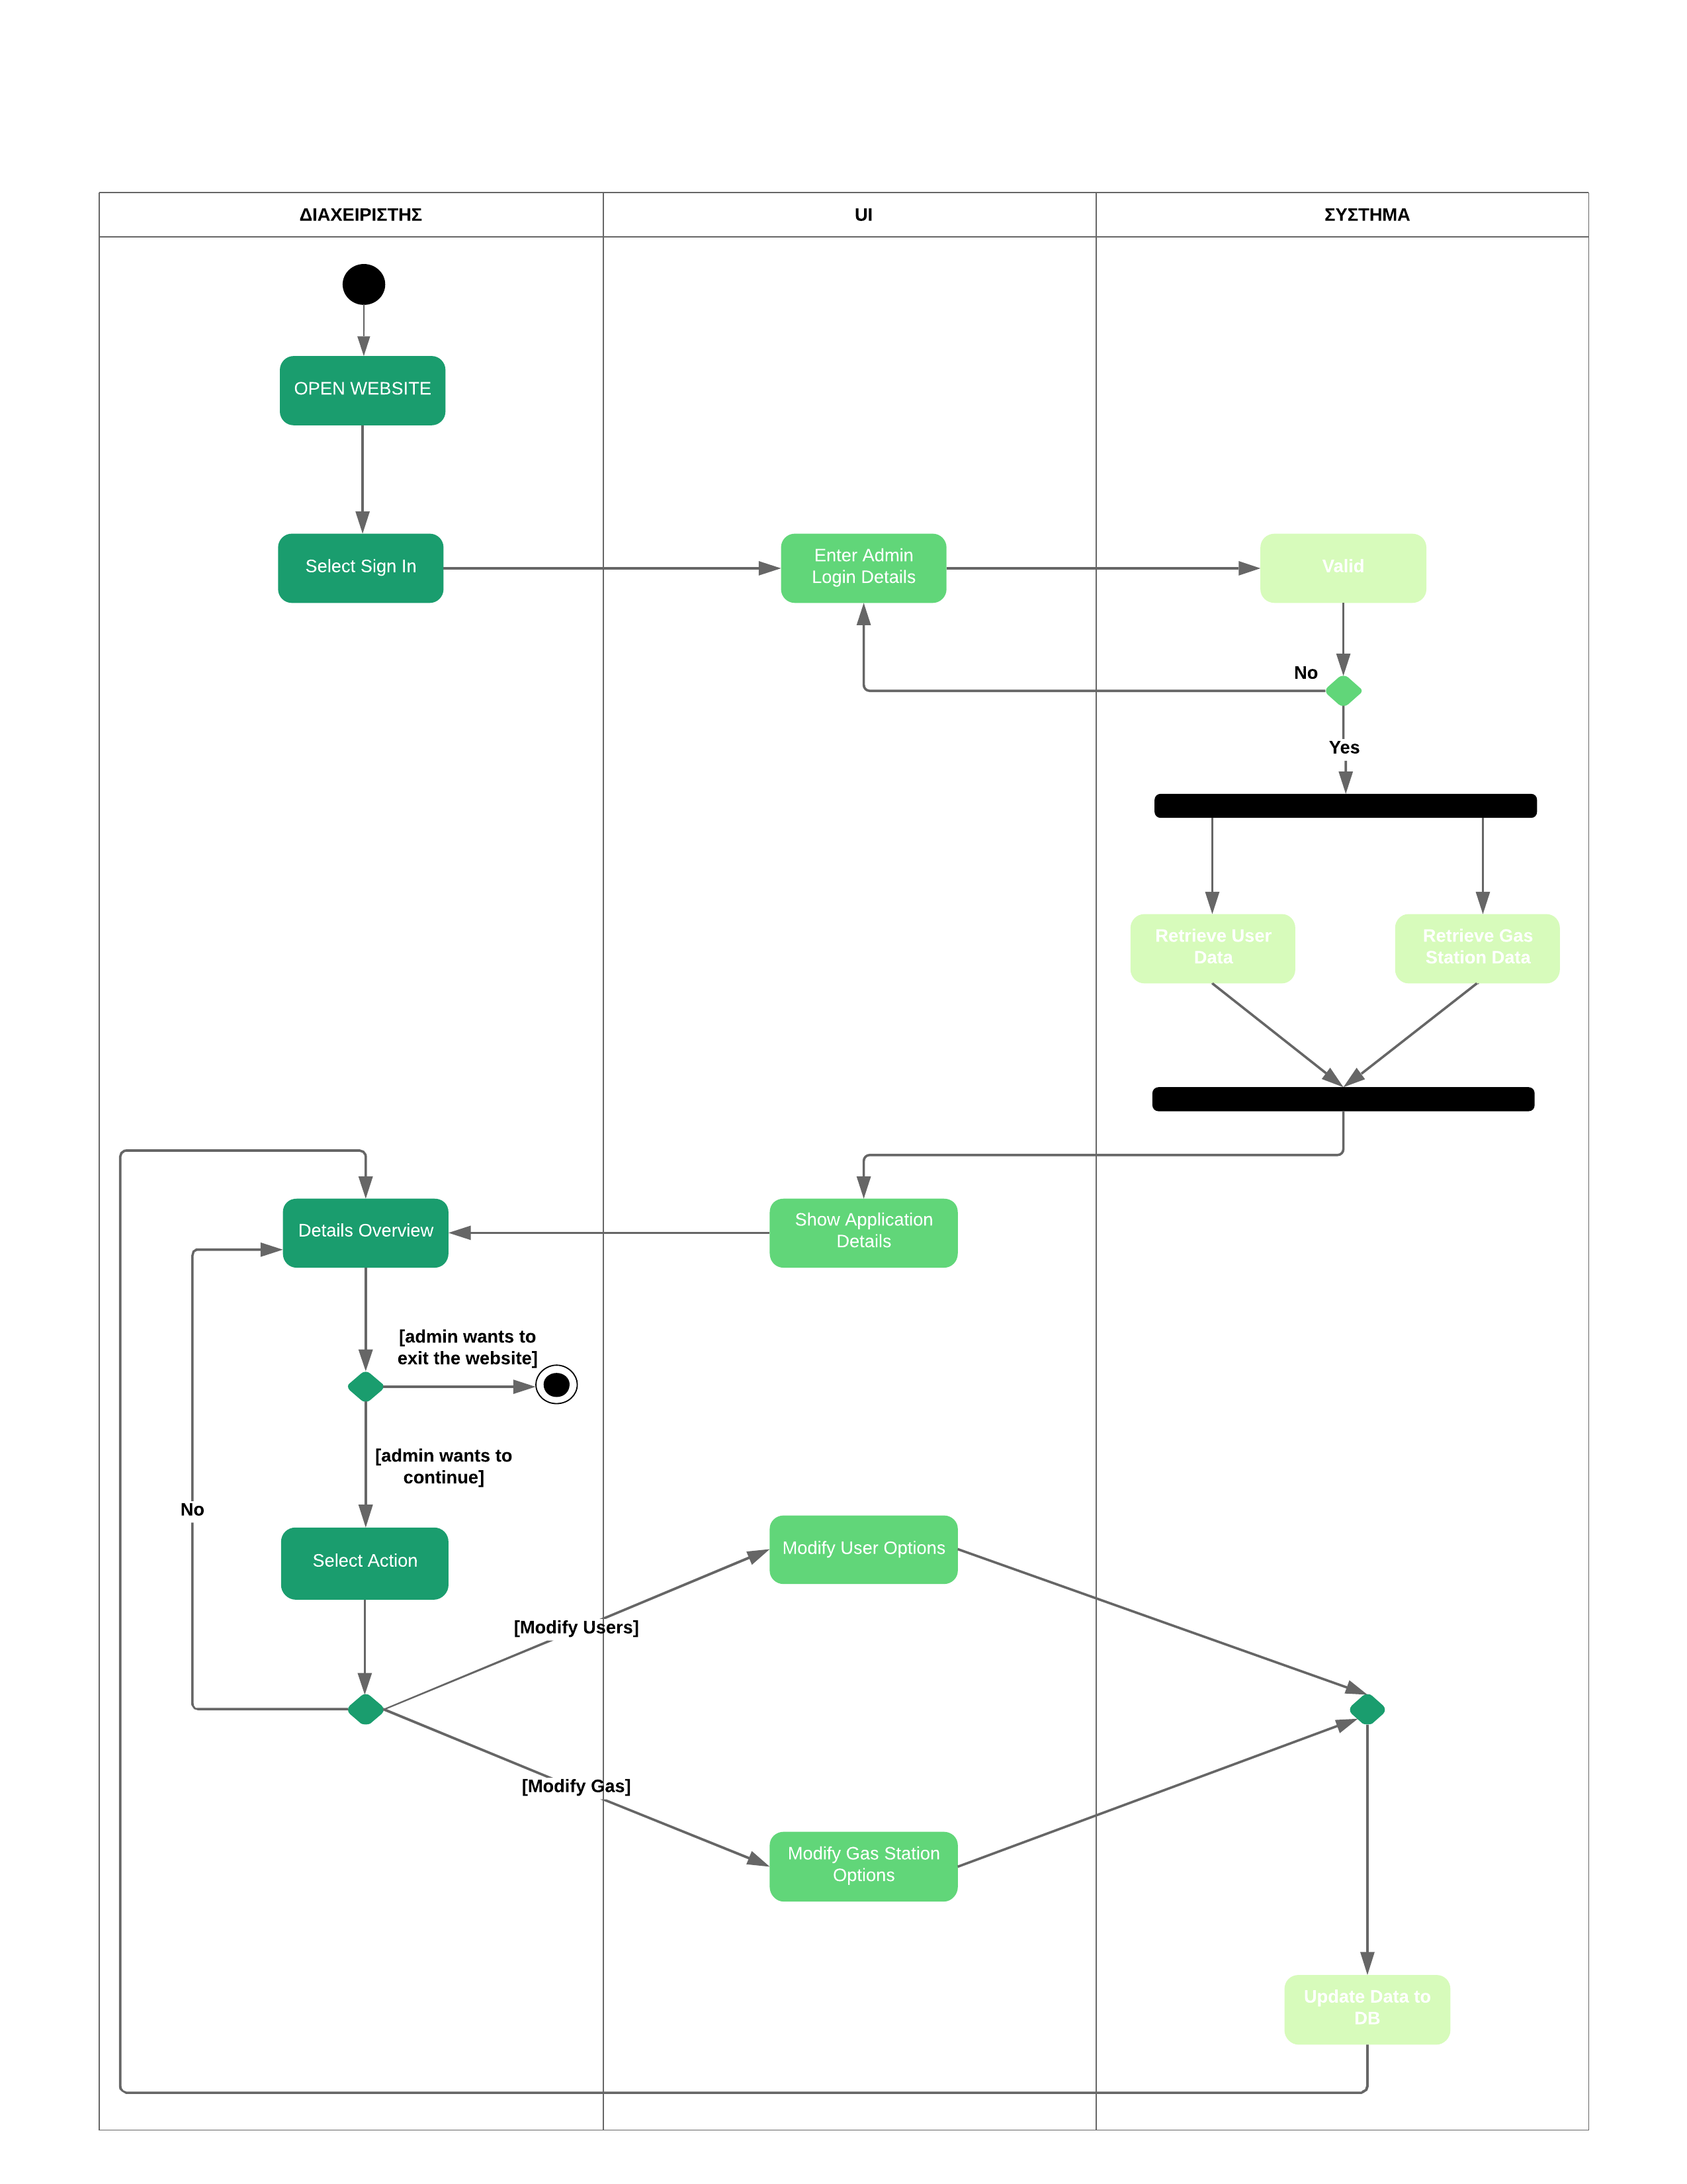
\includegraphics[width = \linewidth]{uml/admin.png}
	\caption{UML activity diagram για \texttt{ΔΙΑΧΕΙΡΙΣΤΗ}}
	\label{admin}
\end{figure}